\documentclass{article}

\thispagestyle{empty}
\usepackage[landscape,scale=.85]{geometry}

\usepackage{amsmath}
\usepackage{fontspec}
\usepackage{unicode-math}
\setmainfont{TeX Gyre Bonum}
\setmathfont{TeX Gyre Bonum Math}

\usepackage{varwidth}

\usepackage{tikz}
\usetikzlibrary{
  matrix,
  matrix.skeleton,
  decorations.pathreplacing,
  calligraphy,
  positioning
}


\ExplSyntaxOn

\seq_new:N \l__linear_seq
\int_new:N \l__term_int
\tl_new:N \l__linear_tl

\DeclareDocumentCommand\LinSeq{s m m m}
{
  \seq_clear:N \l__linear_seq
  \int_set:Nn \l__term_int {#2}
  \seq_put_right:NV \l__linear_seq \l__term_int
  \prg_replicate:nn {#4-1}
  {
    \int_add:Nn \l__term_int {#3}
    \seq_put_right:NV \l__linear_seq \l__term_int
  }
  \IfBooleanTF {#1}
  {
    \seq_pop_left:NN \l__linear_seq \l__linear_tl
    \tl_use:N \l__linear_tl
    \seq_map_inline:Nn \l__linear_seq
    {
      \int_compare:nF {##1 < 0} {+}
      ##1
    }
  }
  {
    \seq_use:Nn \l__linear_seq {,}
  }
}

\DeclareDocumentCommand \Mean {m m}
{
  \int_compare:nTF {\int_mod:nn {#1 + #2}{2} == 0}
  {
    \int_div_truncate:nn {#1 + #2}{2}
  }
  {
    \frac{\int_eval:n {#1 + #2}}{2}
  }
}

\DeclareDocumentCommand \LinSeqnthTerm { m m m }
{
  \int_eval:n {#1 + (#2)*(#3-1)}
}

\DeclareDocumentCommand \LinSeqnthTermRule { m m }
{
  #2 n
  \int_compare:nF {#1 - #2 = 0}
  {
    \int_compare:nT {#1 - #2 > 0} {+}
    \int_eval:n {#1 - #2}
  }
}

\DeclareDocumentCommand \LinSeriesnthSum { m m m }
{
  \int_eval:n {(2*#1 + (#2)*(#3-1))*(#3)/2}
}

\int_new:N \g__random_term_a_int
\int_new:N \g__random_term_b_int
\DeclareDocumentCommand \SetRandoms { m }
{
  \int_compare:nTF {#1 > 6}
  {
    \int_gset:Nn \g__random_term_a_int {\int_rand:nn {5} {#1-1}}
    \bool_do_while:nn
    {
      \int_compare_p:n {\g__random_term_a_int = \g__random_term_b_int}
    }
    {
      \int_gset:Nn \g__random_term_b_int {\int_rand:nn {5} {#1-1}}
    }
  }
  {
    \int_gset:Nn \g__random_term_a_int {6}
    \int_gset:Nn \g__random_term_b_int {7}
  }
  \int_compare:nT {\g__random_term_b_int < \g__random_term_a_int}
  {
    \tl_set:Nx \l_tmpa_tl
    {
      \exp_not:N \int_gset:Nn \exp_not:N \g__random_term_a_int {\int_use:N \g__random_term_b_int}
      \exp_not:N \int_gset:Nn \exp_not:N \g__random_term_b_int {\int_use:N \g__random_term_a_int}
    }
    \tl_use:N \l_tmpa_tl
  }
}

\DeclareDocumentCommand \LinSeqRandomTerm {s m m}
{
  \IfBooleanTF {#1}
  {
    \LinSeqnthTerm {#2}{#3}{\g__random_term_a_int}
  }
  {
    \LinSeqnthTerm {#2}{#3}{\g__random_term_b_int}
  }
}

\DeclareDocumentCommand \LinSeqRandomIndex {s}
{
  \IfBooleanTF {#1}
  {
    \(\int_use:N \g__random_term_a_int\)\Ordinal{\g__random_term_a_int}
  }
  {
    \(\int_use:N \g__random_term_b_int\)\Ordinal{\g__random_term_b_int}
  }
}

\DeclareDocumentCommand \Ordinal {m}
{
  \int_compare:nTF {\int_mod:nn { \int_div_truncate:nn {#1}{10} } {10} = 1}
  {
    th
  }
  {
    \int_case:nnF {\int_mod:nn {#1} {10}}
    {
      {1} {st}
      {2} {nd}
      {3} {rd}
    }
    {th}
  }
}

\cs_new_eq:NN \ampersand \&

\ExplSyntaxOff

  %% First \(4\) terms \&
  %% First term \&
  %% Common difference \&
  %% A random index \&
  %% A random term \&
  %% Another random index \&
  %% Another random term \&
  %% \(n\)th term rule \&
  %% Number of terms \&
  %% Last term \&
  %% Mean of \(1\)st and last \&
  %% Sum of terms \&
\NewDocumentCommand\LinSeqRow {m m m}
{
 \SetRandoms{#3} 
  \(\LinSeq{#1}{#2}{4}\) \&
  \(#1\) \&
  \(#2\) \&
  \LinSeqRandomIndex* \&
  \(\LinSeqRandomTerm*{#1}{#2}\) \&
  \LinSeqRandomIndex \&
  \(\LinSeqRandomTerm{#1}{#2}\) \&
  \(\LinSeqnthTermRule{#1}{#2}\) \&
  \(#3\) \&
  \(\LinSeqnthTerm{#1}{#2}{#3} \) \&
  \(\Mean{#1}{#1 + #2*(#3-1)}\) \&
  \(\LinSeriesnthSum{#1}{#2}{#3}\)
}

\tikzset{
  show cell/.style 2 args={
    row #1 column #2/.style={
      every node/.append style={text opacity=1}
    },
  },
  current row/.initial=1,
  show cell on current row/.style={
    show cell={\pgfkeysvalueof{/tikz/current row}}{#1}
  },
  show cells/.style 2 args={
    current row=#1,
    show cell on current row/.list={#2}
  }
}

\begin{document}

\vspace*{\fill}

\section*{Sequence Completion Grid}

\begin{minipage}{.5\textwidth}
In the following grid:
\begin{itemize}
\item Each row refers to a specific sequence.
\item The paired columns ``Index, Term'' refer to a specific term in the sequence; the ``index'' is \emph{where} it is and the \emph{term} is its value.
\item The last four columns are about summing a specific number of terms of the sequence, starting from the first term.
The ``last term'' is the last term in the sum.
\end{itemize}
\end{minipage}

\vspace*{\fill}


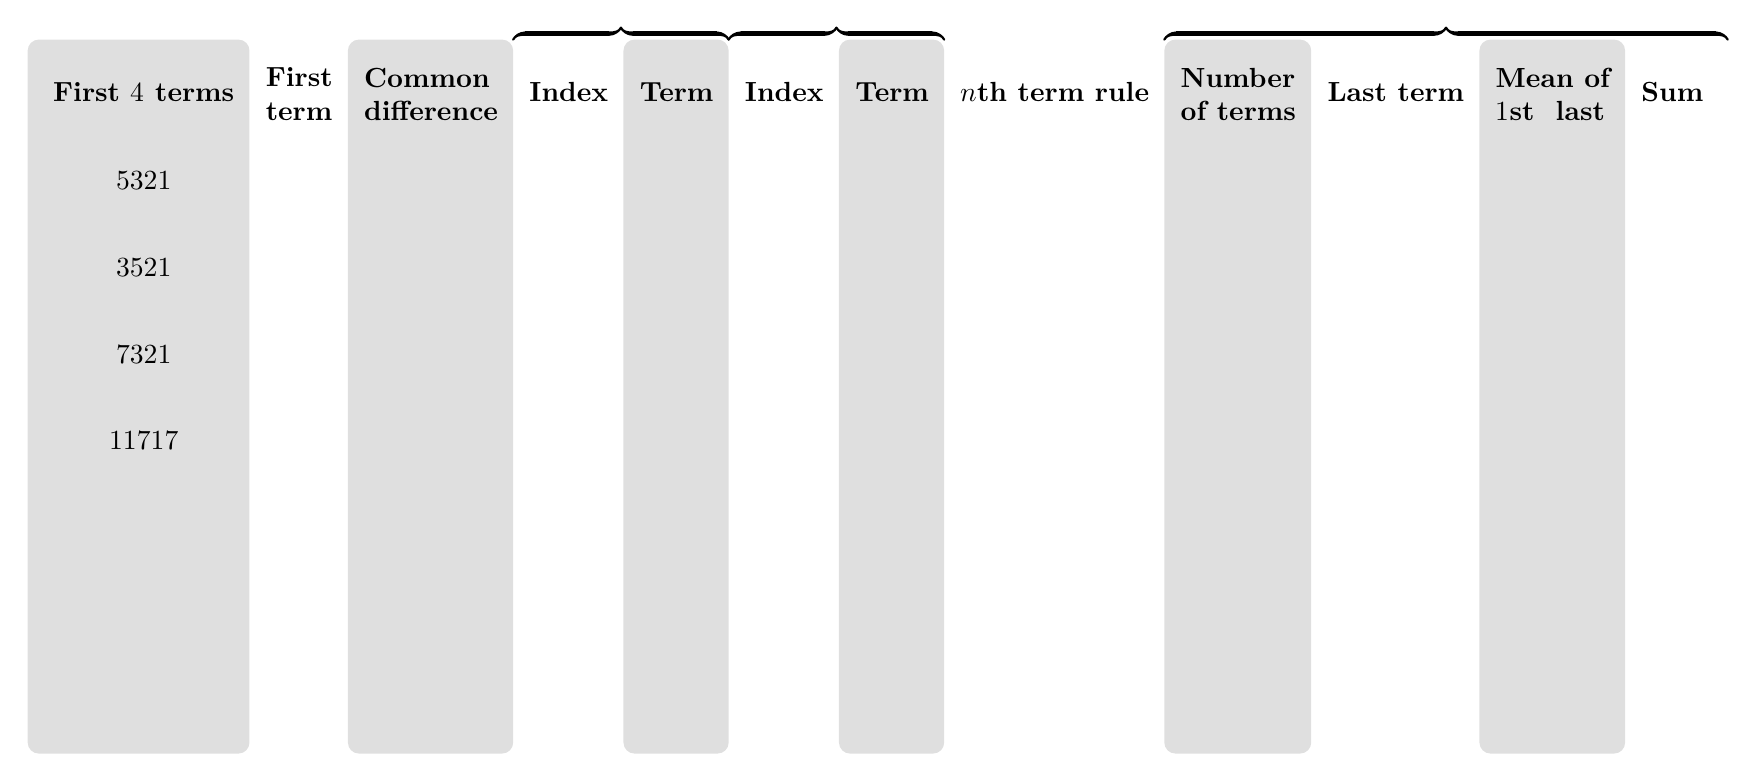
\begin{tikzpicture}
\matrix[
  matrix of nodes,
  ampersand replacement=\&,
  nodes={inner xsep=2mm, minimum width=.8cm,text opacity=0,minimum height=1.1cm},
  row 1/.style={every node/.append style={font=\bfseries,text opacity=1}},
  style odd tiling columns={fill=gray!25,rounded corners},
  %
  row 2/.style={every node/.append style={text opacity=1}},
  %
  show cells={3}{1,4,6,9},
  show cells={4}{1,4,6,9},
  show cells={5}{1,5,7,10},
  show cells={6}{4,5,6,7},
  show cells={7}{4,6,8,9},
  show cells={8}{2,5,7,10,12},
]
(m)
{
  First \(4\) terms \&
  \begin{varwidth}{1in}First\\term\end{varwidth} \&
  \begin{varwidth}{1in}Common\\difference\end{varwidth} \&
  Index \&
  Term \&
  Index \&
  Term \&
  \(n\)th term rule \&
  \begin{varwidth}{1in}Number\\of terms\end{varwidth} \&
  Last term \&
  \begin{varwidth}{1in}Mean of\\\(1\)st \ampersand\ last\end{varwidth} \&
  Sum
  \\
  \LinSeqRow{5}{3}{21}  \\ % 2
  \LinSeqRow{3}{5}{21}  \\ % 3
  \LinSeqRow{7}{3}{21}  \\ % 4
  \LinSeqRow{11}{7}{17}  \\ % 5
  \LinSeqRow{3}{2}{19} \\ % 6
  \LinSeqRow{8}{5}{32} \\ % 7
  \LinSeqRow{13}{4}{14} \\ % 8
};

\draw[
  decorate,
  decoration={calligraphic brace,amplitude=1ex},
  ultra thick
] (m-tiling-cell-1-4.north west) -- (m-tiling-cell-1-5.north east);
\draw[
  decorate,
  decoration={calligraphic brace,amplitude=1ex},
  ultra thick
] (m-tiling-cell-1-6.north west) -- (m-tiling-cell-1-7.north east);
\draw[
  decorate,
  decoration={calligraphic brace,amplitude=1ex},
  ultra thick
] (m-tiling-cell-1-9.north west) -- (m-tiling-cell-1-12.north east);
\end{tikzpicture}

\vspace*{\fill}


\end{document}
